%----------------------------------------------------------------------
\begin{frame}[c]{Where are we? The big picture}

\begin{itemize}
\item Algorithm Selection
  \begin{itemize}
    \item Portfolios
    \item Algorithm selection (for runtime)
  \end{itemize}
  \item Design decisions:\\ Local Search + Evo. Algorithms + Machine Learning 
  \item Empirical evaluation
  \item AAD for ML
  \begin{itemize}
    \item Hyperparameter optimization and Bayesian optimization 
    \item Neural architecture search (lecture given by Prof. Hutter)
  \end{itemize}
  \item Algorithm configuration 
  \begin{itemize}
    \item Basics 
    \item State of the art 
    \item Best practices 
  \end{itemize}
  \item Combinations of algorithm selection and configurations
  \item[$\to$] Algorithm control and learning to learn
  \item Algorithm analysis 
  \item Project announcement and questions for exam 
\end{itemize}

\end{frame}
%----------------------------------------------------------------------
%----------------------------------------------------------------------
\begin{frame}[c]{Learning Goals}

After this lecture, you will be able to \ldots

\begin{itemize}
  \item motivate and define the algorithm control problem
  \item list challenges in algorithm control
  \item explain how reinforcement learning can be used for algorithm control
  \item explain the idea behind learning to   
  \begin{itemize}
    \item learn by gradient descent by gradient descent
    \item optimize black box functions
    \item optimize via reinforcement learning
  \end{itemize}
\end{itemize}

\end{frame}
%----------------------------------------------------------------------
%----------------------------------------------------------------------
\begin{frame}[c]{Reminder: Algorithm Configuration}

\includegraphics[width=0.9\textwidth]{images/ac_comic}

\pause

\bigskip
$\leadsto$ \alert{We set the configuration once and\\ use it for the entire run of an algorithm}\\
$\leadsto$ \alert{Black box view on algorithm}
\end{frame}
%----------------------------------------------------------------------
%----------------------------------------------------------------------
\begin{frame}[c]{Dynamic Heuristics}

\begin{itemize}
  \item Many heuristics in algorithms are dynamic and adaptive
  \begin{enumerate}
    \item the algorithm's behavior changes over time
    \item the algorithm's behavior changes based on internal statistics
  \end{enumerate}
  \medskip
  \item these heuristics might control other parameters of the algorithms
  \pause
  \smallskip
  \item example: learning rate schedules for training DNNs
  \begin{enumerate}
  	\item exponential decaying learning rate: based on number of iterations, learning rate decreases
  	\pause
  	\item Reduce learning rate on plateaus: if the learning stagnates for some time, the learning rate is decreased by a factor
  \end{enumerate}
  \pause
  \item What examples for dynamic heuristics can you think of? \hands
  \pause
  \item other examples: restart probability of SLS solvers, mutation rate of evolutionary algorithms, \ldots  
  
\end{itemize}

\end{frame}
%----------------------------------------------------------------------
%----------------------------------------------------------------------
\begin{frame}[c]{Parametrization of Learning Rate Schedules}

\begin{itemize}
  \item How would we parameterize learning rate schedules?
  \begin{enumerate}
  	\item exponential decaying learning rate:
  	\begin{itemize}
  	  \item initial learning rate
  	  \item minimal learning rate
  	  \item multiplicative factor
  	\end{itemize}
  	\pause
  	\item Reduce learning rate on plateaus:
  	\begin{itemize}
  	  \item patience (in number of epochs)
  	  \item patience threshold
  	  \item decreasing factor
  	  \item cool-down break (in number of epochs)
  	\end{itemize}
  \end{enumerate}
  \pause
  \medskip
  \item[$\leadsto$] Many parameters only to control a single parameter (learning rate)
  \pause   
  \item Still not guaranteed that optimal setting of learning rate schedules will lead to optimal learning rate behavior
  \begin{itemize}
    \item Learning rate schedules are only heuristics
  \end{itemize}
\end{itemize}

\end{frame}
%----------------------------------------------------------------------
%----------------------------------------------------------------------
\begin{frame}[c]{Algorithm Control}

\begin{block}{Idea Algorithm Control}
Can we \alert{learn from empirical data} how to set algorithm parameters dynamically in the course of running the algorithm?
\pause
\begin{itemize}
  \item Essentially, learning of dynamic heuristics
\end{itemize}
\end{block}

\pause

\begin{block}{Algorithm Control: \textbf{Simplified} Definition}
Formally, given
\begin{itemize}
  \item a parameterized algorithm $\algo$ with a configuration space $\pcs$,
  \pause
  \item a state description $\state_t \in \states$ of algorithm $\algo$ at each time point~$t$,
  \pause
  \item a space of possible control policies $\policies: \states \to \pcs$, and
  \pause
  \item a cost metric $c: \policies \to \mathbb{R}$ assessing the cost of a control policy $\policy \in \policies$,
\end{itemize}

\noindent the goal is to obtain a well-performing \emph{control policy}: $\policy^* \in \argmin_{\policy \in \policies} c(\policy)$.
\end{block}

\end{frame}
%----------------------------------------------------------------------
%----------------------------------------------------------------------
\begin{frame}[c]{Setting in Algorithm Control}

\begin{block}{General Setting}
\begin{itemize}
  \item Offline phase: 
  \begin{itemize}
    \item gather performance data $c(\policy)$ for different policies
    \item find well-performing policy $\policy^*$
  \end{itemize}
  \item Online phase: apply $\policy^*$
\end{itemize}
\end{block}

\medskip

\includegraphics[width=1.\textwidth]{images/algorithm_control_comic}

\end{frame}
%----------------------------------------------------------------------
%----------------------------------------------------------------------
\begin{frame}[c]{Supervised Learning for Algorithm Control}


\begin{block}{Idea 1: Supervised Learning for Algorithm Control}
\begin{itemize}
  \item Algorithm control can be modelled as a supervised learning problem,\\ since we want to learn $\policies: \states \to \pcs$
  \item Approach:
  \begin{enumerate}
    \item gather performance data $c(\policy)$ for different policies: $ \conf_t \times \state_t \mapsto y$
    \pause
    \item learn mapping $q: \pcs \times \states \to \perf$ (e.g., by using DNNs)
    \pause
    \item Online: policy $\policy: \conf_t \in \argmin_{\conf \in \pcs} q(\conf, \state_t)$ at $\state_t$
  \end{enumerate}
  \medskip
  \pause
  \item Why won't that work well? \hands
  \pause
  \item Problems:
  \begin{itemize}
    \item Training data is not independent and identically distributed (i.i.d)\\
    because $s_t$ depends on $s_{t+1}$ 
    \begin{itemize}
      \item[$\leadsto$] Possible approach: recurrent neural networks (RNNs) 
    \end{itemize}
    \pause
    \item How should we sample policies $\policy$ to gather training data?
    \begin{itemize}
      \item[$\leadsto$] Possible approach: observe existing hand-designed heuristics
    \end{itemize}
  \end{itemize}
\end{itemize}
\end{block}

\end{frame}
%----------------------------------------------------------------------
%----------------------------------------------------------------------
\begin{frame}[c]{Reinforcement Learning for Algorithm Control}


\begin{block}{Idea 2: Reinforcement Learning for Algorithm Control}
\begin{itemize}
  \item Algorithm control is an inherent sequential decision making problem
  \begin{description}
  	\item[Environment:] Algorithm
  	\item[Action:] change of parameter settings
  	\item[State:] state of algorithm
  	\item[Reward:] performance (or negative cost)
  	\item[Episode:] A run of the algorithm
  \end{description}
\end{itemize}

\pause

\medskip
\centering
\scalebox{0.8}{\tikzstyle{activity}=[rectangle, draw=black, rounded corners, text centered, text width=6em, fill=white, drop shadow]
\tikzstyle{data}=[rectangle, draw=black, text centered, fill=black!10, text width=8em, drop shadow]
\tikzstyle{myarrow}=[->, thick]
\begin{tikzpicture}[node distance=10em]
	
	
	\node (agent) [activity] {Agent};
	\node (environment) [activity, below of=agent, node distance=6em] {Environment};
	
	\draw[thick] (agent) -- ($(agent.east)+(1,0)$);
	\draw[thick] ($(agent.east)+(1,0)$) -- ($(environment.east)+(1,0)$) node [left,yshift=3em] {Action $a_t$};
	\draw[myarrow] ($(environment.east)+(1,0)$) -- (environment);
	
	\draw[thick] (environment) -- ($(environment.west)+(-1,0)$);
	\draw[thick] ($(environment.west)+(-1,0)$) -- ($(agent.west)+(-1,0)$) node [right,yshift=-3em] {State $s_{t}$};
	\draw[myarrow] ($(agent.west)+(-1,0)$) -- (agent);
	
	\draw[thick] ($(environment.west)+(0,-0.15)$) -- ($(environment.west)+(-1.15,-0.15)$);
	\draw[thick] ($(environment.west)+(-1.15,-0.15)$) -- ($(agent.west)+(-1.15,0.15)$) node [left,yshift=-3.4em] {Reward $r_{t}$};
	\draw[myarrow] ($(agent.west)+(-1.15,0.15)$) -- ($(agent.west)+(0,0.15)$);
	
	\draw[thick] ($(environment.west)+(-0.8,-0.35)$) -- ($(environment.west)+(-0.8,0.2)$);
	
	\draw[myarrow] ($(environment.west)+(0,-0.15)$) -- ($(environment.west)+(-0.8,-0.15)$) node [below, xshift=1.1em] {$r_{t+1}$};
	\draw[myarrow] ($(environment.west)+(0,-0.0)$) -- ($(environment.west)+(-0.8,-0.0)$) node [above, xshift=1.1em] {$s_{t+1}$};
	
\end{tikzpicture}

\tikzstyle{activity}=[rectangle, draw=black, rounded corners, text centered, text width=6em, fill=white, drop shadow]
\tikzstyle{data}=[rectangle, draw=black, text centered, fill=black!10, text width=8em, drop shadow]
\tikzstyle{myarrow}=[->, thick]
\begin{tikzpicture}[node distance=10em]
	
	
	\node (agent) [activity, text width=8em] {Control Policy~$\policy$};
	\node (environment) [activity, below of=agent, node distance=6em, text width=8em] {Algorithm};
	
	\draw[thick] (agent) -- ($(agent.east)+(1,0)$);
	\draw[thick] ($(agent.east)+(1,0)$) -- ($(environment.east)+(1,0)$) node [left,yshift=3em] {Configuration $\conf_t$};
	\draw[myarrow] ($(environment.east)+(1,0)$) -- (environment);
	
	\draw[thick] (environment) -- ($(environment.west)+(-1,0)$);
	\draw[thick] ($(environment.west)+(-1,0)$) -- ($(agent.west)+(-1,0)$) node [right,yshift=-3em] {State $\state_t(i)$};
	\draw[myarrow] ($(agent.west)+(-1,0)$) -- (agent);
	
	\draw[thick] ($(environment.west)+(0,-0.15)$) -- ($(environment.west)+(-1.15,-0.15)$);
	\draw[thick] ($(environment.west)+(-1.15,-0.15)$) -- ($(agent.west)+(-1.15,0.15)$) node [left,yshift=-3.4em] {Cost $c_t$};
	\draw[myarrow] ($(agent.west)+(-1.15,0.15)$) -- ($(agent.west)+(0,0.15)$);
	
	\draw[thick] ($(environment.west)+(-0.8,-0.35)$) -- ($(environment.west)+(-0.8,0.2)$);
	
	\draw[myarrow] ($(environment.west)+(0,-0.15)$) -- ($(environment.west)+(-0.8,-0.15)$) node [below, xshift=1.1em] {$c_{t+1}$};
	\draw[myarrow] ($(environment.west)+(0,-0.0)$) -- ($(environment.west)+(-0.8,-0.0)$) node [above, xshift=1.1em] {$\state_{t+1}$};
	
\end{tikzpicture}
}

Reinforcement learning \hspace{1.4cm} Algorithm Control 

\end{block}

\end{frame}
%----------------------------------------------------------------------
%----------------------------------------------------------------------
\begin{frame}[c]{State Description}

\begin{itemize}
  \item State description are conceptually similar to instance features
  \item Should describe recent state of the algorithm
  \medskip
  \pause
  \item Examples of state descriptions:
  \begin{itemize}
    \item Control of learning rate:
    \begin{itemize}
      \item loss improvement of the last updates
      \item current gradient
      \item previous learning rates
    \end{itemize}
    \item SLS solvers:
    \begin{itemize}
      \item improvement of incumbent ($\#$unsatisfied clauses) in the last steps
      \item distance in the solution space  
    \end{itemize}
  \end{itemize}
  \medskip
  \pause
  \item Important characteristics:
  \begin{itemize}
    \item cheap-to-compute!\\ (computed not only in the beginning but several time during solving)
    \item informative wrt the progress of the algorithm
  \end{itemize}
\end{itemize}

\end{frame}
%----------------------------------------------------------------------
%----------------------------------------------------------------------
\begin{frame}[c]{Can we learn Algorithm control? (SLS example)}

\includegraphics[width=0.9\textwidth]{images/THE_BAD_Selman-sel_2000_8400_2}

\pause
$\leadsto$ On some instances (without much structure), we were not able\\ to find a better policy than a static configuration.

\end{frame}
%----------------------------------------------------------------------
%----------------------------------------------------------------------
\begin{frame}[c]{Can we learn Algorithm control? (SLS example)}

\includegraphics[width=0.9\textwidth]{images/THE_GOOD_Engine6-engine_6_nd_case1-zoomed}

\pause
$\leadsto$ On some instances (with structure), algorithm control outperforms\\ algorithm configuration.

\end{frame}
%----------------------------------------------------------------------
%----------------------------------------------------------------------
\begin{frame}[c]{Algorithm Control across Instances}

\begin{itemize}
  \item As in algorithm configuration, algorithm control policies should perform well across instances
\end{itemize}

\begin{block}{Algorithm Control \textbf{Full} Definition}
Formally, given
\begin{itemize}
  \item a parameterized algorithm $\algo$ with a configuration space $\pcs$,
  \pause
  \item a state description $\state_t \in \states$ of algorithm $\algo$ at each time point~$t$,
  \pause
  \item \alert{a set of instances $\insts$,}
  \pause
  \item a space of possible control policies $\policies: \states \to \pcs$, and
  \pause
  \item a cost metric $c: \policies \times \insts \to \mathbb{R}$ assessing the cost of a control policy $\policy \in \policies$ on a given instance $\inst \in \insts$,
\end{itemize}

\noindent the goal is to obtain a well-performing \emph{control policy} across all instances: $\policy^* \in \argmin_{\policy \in \policies} \sum_{\inst \in \insts}c(\policy, \inst)$.
\end{block}

\end{frame}
%----------------------------------------------------------------------
%----------------------------------------------------------------------
\begin{frame}[c]{Generalization of Algorithm Control?}

\begin{itemize}
  \item Open problem: how well will algorithm control generalize to new $\insts_{\text{test}}$
  \begin{enumerate}
    \item algorithm control allows to control algorithms even more and\\ thus, the chance of over-tuning increases
    \pause
    \item algorithm control learns (e.g. by using DNNs) mappings $\policies: \states \to \pcs$ which use more information than static configurations
  \end{enumerate}
  \pause
  \item prevent that learned $\policy$ will implicitly learn solution of a given $\inst$ 
  \pause
  \medskip
  \item Possible cases
  \begin{itemize}
    \item Learned policy generalizes to similar, homogeneous instances
    \begin{itemize}
      \item can hopefully be learned from state information
    \end{itemize}
    \item Learned policy might consider instance features $\policies: \states \times \feats \to \pcs$\\ and generalize also to heterogeneous instances
  \end{itemize}  
  \pause
  \item Example~\lit{Daniel et al. AAAI'16}:  controller for learning rates\\ for training deep neural networks
  \begin{itemize}
    \item for training controller, sample DNN architecture and data subsets 
  \end{itemize}
  \pause
  \item[$\leadsto$] Open research topic how to do it efficiently and at scale!
\end{itemize}

\end{frame}
%----------------------------------------------------------------------
%----------------------------------------------------------------------
\begin{frame}[c]{Learning to Learn}

\begin{block}{Idea}
\begin{itemize}
  \item Learn algorithms directly, i.e., how to search in the solution space
  \item First idea: learn weight updates of a neural network\\
  (not only the learning rate)
\end{itemize}
\end{block}

\pause

\begin{block}{Learning to learn by gradient descent by gradient descent\newline \litw{Andrychowicz et al'16}}
Weight updates (note: \alert{$\theta$ denote DNN weights!}):
\begin{equation}
\theta_{t+1} = \theta_t - \alpha_t \nabla f(\theta_t) \nonumber
\end{equation}
\pause
Even more general:
\begin{equation}
\theta_{t+1} = \theta_t + g_t(\nabla f(\theta_t), \phi) \nonumber
\end{equation}
where $g$ is the optimizer and $\phi$ are the parameters of the optimizer $g$.\\
\pause
$\leadsto$ \alert{Goal: Optimize $f$ wrt $\theta$ by learning $g$}
\end{block}

\end{frame}
%----------------------------------------------------------------------
%----------------------------------------------------------------------
\begin{frame}[c]{Learning to Learn: Objective\newline \litw{Andrychowicz et al'16}}

\vspace{-0.5cm}
\begin{equation}
\mathcal{L}(\phi) = \mathbb{E}\left[ f(\theta^*(f,\phi)) \right]\nonumber
\end{equation}

where $\mathcal{L}$ is a loss function and $\theta^*(f,\phi)$ are the optimized weights $\theta^*$ by using the optimizer parameterized with $\phi$ on function $f$.

\pause

%\vspace{-0.5cm}
\begin{equation}
\mathcal{L}(\phi) = \mathbb{E}\left[\sum_{t=1}^T w_t f(\theta_t)\right]\nonumber
\end{equation}

\pause
where $w_t$ are arbitrary weights associated with each time step
and 

\pause
\vspace{-0.5cm}
\begin{eqnarray}
\theta_{t+1} = \theta_t + g_t\\\nonumber
\begin{pmatrix}g_t\\h_{t+1}\end{pmatrix} = m(\nabla_\theta f(\theta_t), h_t, \phi)\nonumber
\end{eqnarray}

\pause
$\leadsto$ Goal: Learn $m$ via $\phi$ by using gradient descent by optimizing $\mathcal{L}$ \\
\pause
$\leadsto$ ``Learning to learn gradient descent by gradient descent''
\end{frame}
%----------------------------------------------------------------------
%----------------------------------------------------------------------
\begin{frame}[c]{Learning to Learn: LSTM approach\newline \litw{Andrychowicz et al'16}}

\begin{description}
	\item[Optimizee] Target network to be trained
	\item[Optimizer] LSTM with hidden state $h_t$ that predicts weight updates $g_t$
\end{description}

\medskip

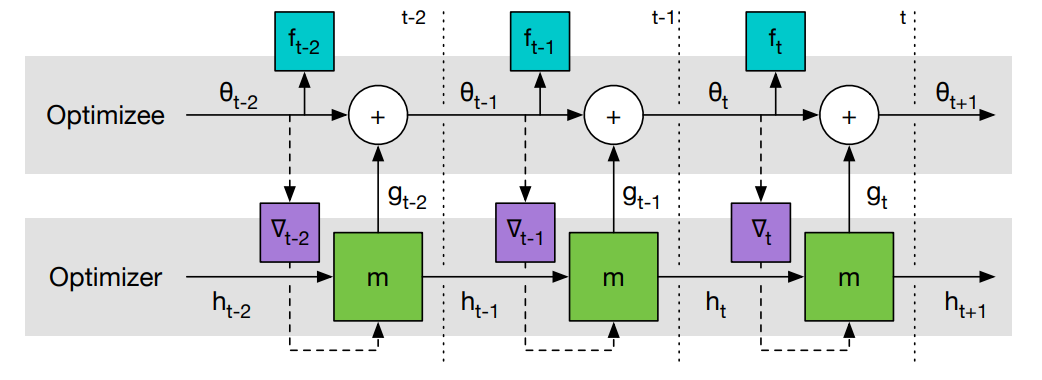
\includegraphics[width=1\textwidth]{images/learning_to_learn_lstm}

\end{frame}
%----------------------------------------------------------------------
%----------------------------------------------------------------------
\begin{frame}[c]{Learning to Learn with LSTM: Results\newline \litw{Andrychowicz et al'16}}

\centering
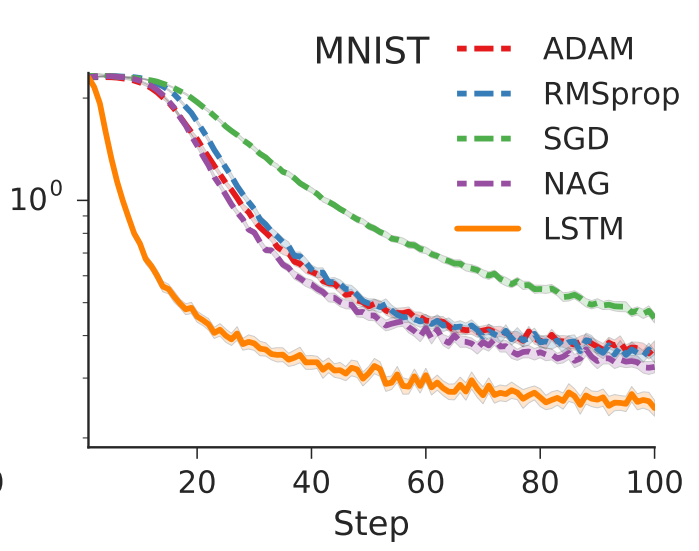
\includegraphics[width=0.7\textwidth]{images/l2l_mnist_base}

\end{frame}
%----------------------------------------------------------------------
%----------------------------------------------------------------------
\begin{frame}[c]{Learning to Learn with LSTM: Results\newline \litw{Andrychowicz et al'16}}

Changing the original architecture of the DNN:
\smallskip

\centering
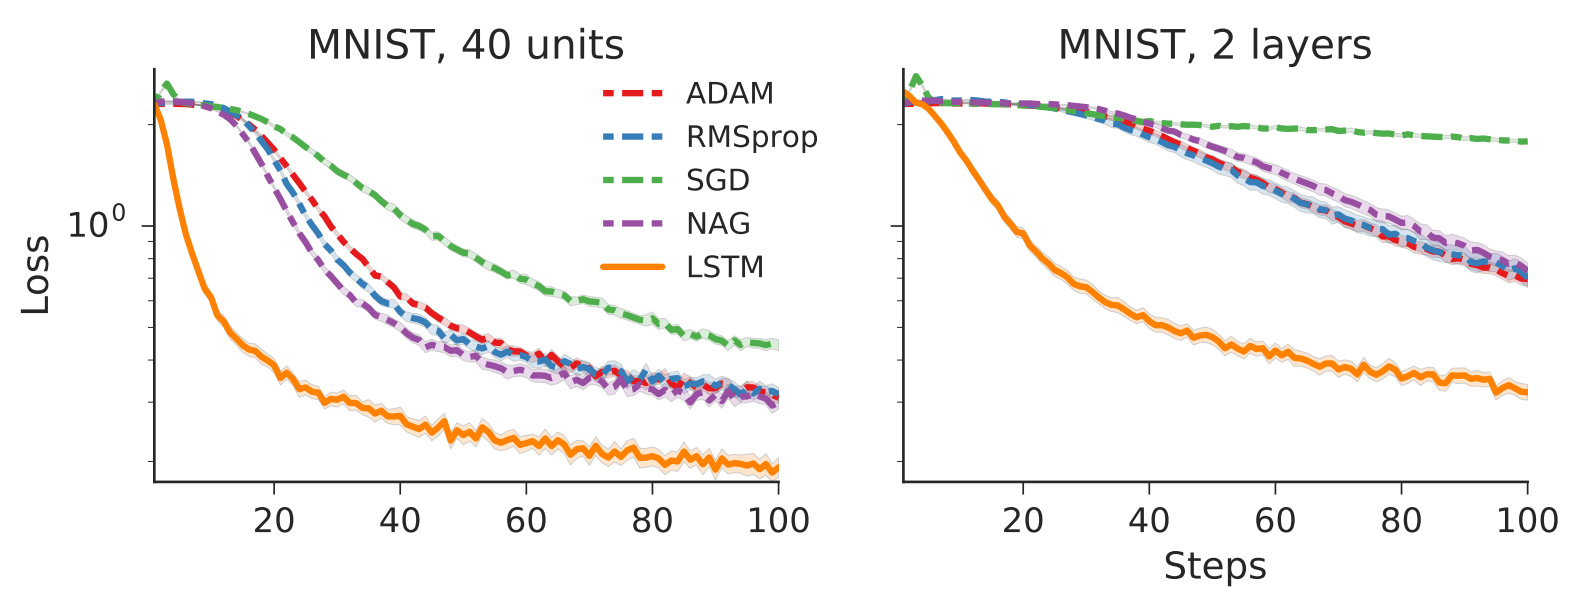
\includegraphics[width=0.9\textwidth]{images/l2l_mnist_okchange}

$\leadsto$ learnt optimizer is robust against some architectural changes

\end{frame}
%----------------------------------------------------------------------
%----------------------------------------------------------------------
\begin{frame}[c]{Learning to Learn with LSTM: Results\newline \litw{Andrychowicz et al'16}}

Changing the activation function to ReLU:
\smallskip

\centering
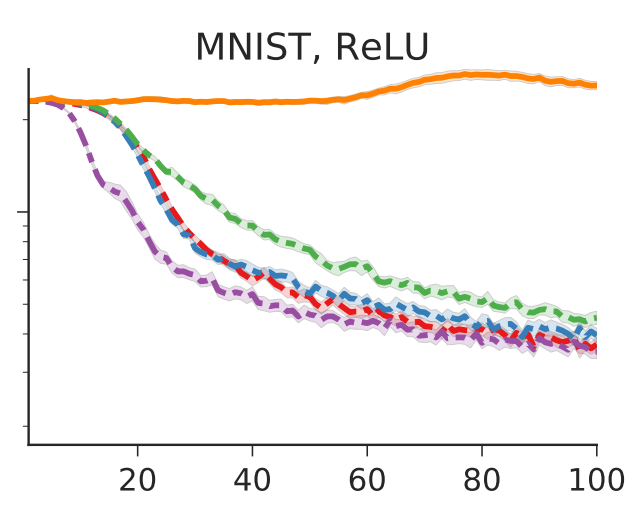
\includegraphics[width=0.6\textwidth]{images/l2l_mnist_relu}

$\leadsto$ fails on other activation functions

\end{frame}
%----------------------------------------------------------------------
%----------------------------------------------------------------------
\begin{frame}[c]{Learning Black-box Optimization~\litw{Chen et al'17}}

\begin{block}{Black Box Optimization Setting}
\begin{enumerate}
  \item Given the current state of knowledge $h_t$ propose a query point $x_t$
  \item Observe the response $y_t$
  \item Update any internal statistics to produce $h_{t+1}$
\end{enumerate}
\end{block}

\pause

\begin{block}{Learning Black Box Optimization}
Essentially, same idea as before:
\begin{eqnarray}
h_t, x_t = \text{RNN}_\phi(h_{t-1}, x_{t-1}, y_{t-1}) \nonumber \\
y_t \sim p(y|x_t)\nonumber
\end{eqnarray}

\begin{itemize}
  \item Using recurrent neural network (RNN) to predict next $x_t$.
  \item $h_t$ is the internal hidden state 
\end{itemize}

\end{block}



\end{frame}
%----------------------------------------------------------------------
%----------------------------------------------------------------------
\begin{frame}[c]{Learning Black-box Optimization: Loss Functions\newline \litw{Chen et al'17}}

\begin{itemize}
  \item Sum loss: Provides more information than final loss
\end{itemize}
\begin{equation}
\mathcal{L}_{\text{sum}}(\phi) = \mathbb{E}_{f,y_{1:T-1}}\left[\sum_{t=1}^T f(x_t)\right]\nonumber
\end{equation}

\pause

\begin{itemize}
  \item EI loss: Try to learn behavior of Bayesian optimizer based on expected improvement (EI)
  \begin{itemize}
    \item requires model (e.g., GP)
  \end{itemize}
\end{itemize}
\begin{equation}
\mathcal{L}_{\text{EI}}(\phi) = - \mathbb{E}_{f,y_{1:T-1}}\left[\sum_{t=1}^T \text{EI}(x_t | y_{1:t-1})\right]\nonumber
\end{equation}

\pause

\begin{itemize}
  \item Observed Improvement Loss:
\end{itemize}

\begin{equation}
\mathcal{L}_{\text{OI}}(\phi) = \mathbb{E}_{f,y_{1:T-1}}\left[\sum_{t=1}^T \min \left\{f(x_t) - \min_{i<t}(f(x_i)),0 \right\}  \right]\nonumber
\end{equation}

\end{frame}
%----------------------------------------------------------------------
%----------------------------------------------------------------------
\begin{frame}[c]{Learning Black-box Optimization: Results\newline \litw{Chen et al'17}}

\centering
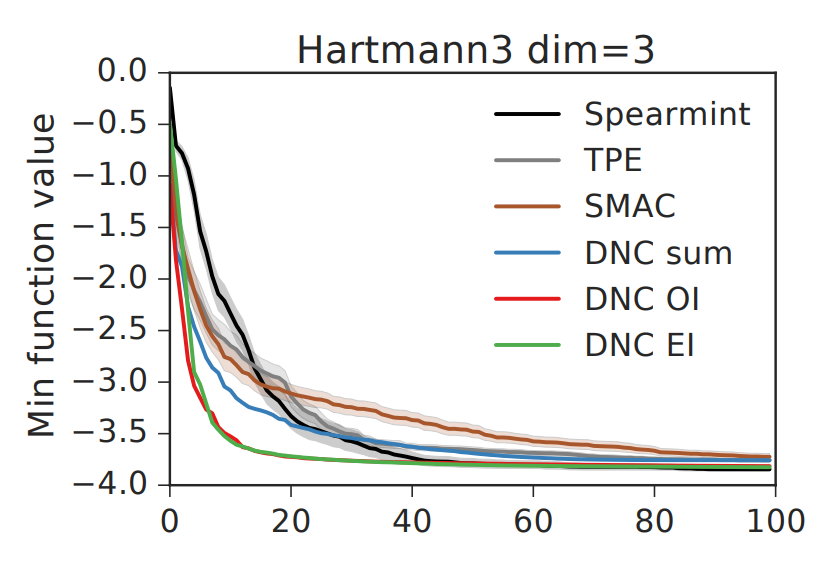
\includegraphics[width=0.7\textwidth]{images/l2bo_hartmann3}

\begin{itemize}
  \item Hartmann3 is an artifical function with 3 dimensions
  \pause
  \item[$\leadsto$] $\mathcal{L}_{\text{OI}}$ and $\mathcal{L}_{\text{EI}}$ perform best
  \item[$\leadsto$] $\mathcal{L}_{\text{OI}}$ easier to compute than $\mathcal{L}_{\text{EI}}$ 
\end{itemize}

\end{frame}
%----------------------------------------------------------------------
%----------------------------------------------------------------------
\begin{frame}[c]{Learning to Optimize via Reinforcement Learning\newline \litw{Li and Malik'17}}

\centering
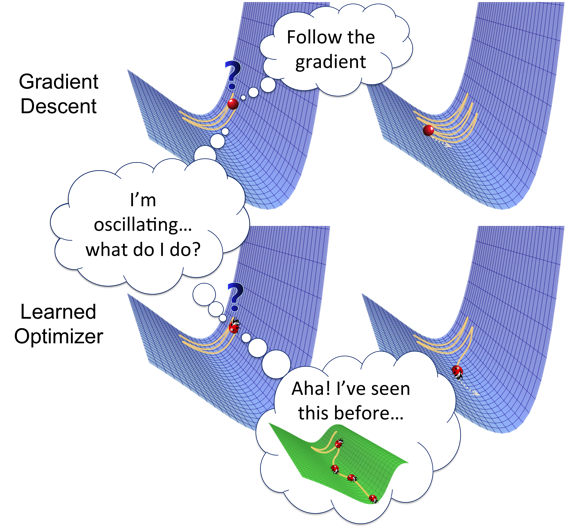
\includegraphics[width=0.6\textwidth]{images/l2o_comic}

\tiny
Source: \url{https://bair.berkeley.edu/blog/2017/09/12/learning-to-optimize-with-rl/}

\end{frame}
%----------------------------------------------------------------------
%----------------------------------------------------------------------
\begin{frame}[c]{Learning to Optimize via Reinforcement Learning\newline \litw{Li and Malik'17}}

\begin{block}{Reinforcement Learning for Learning to Optimize}
\begin{description}
	\item[State] current location, objective values and gradients evaluated at the current and past locations
	\pause
	\item[Action] Step update $\Delta x$
	\pause
	\item[Transition] $x_t \leftarrow x_{t-1} + \Delta x$
	\pause
	\item[Cost/Reward] Objective value at the current location
	\begin{itemize}
	  \item Since the RL agent will optimize the cumulative cost, this is equivalent to $\mathcal{L}_{\text{sum}}$
	  \item encourages the policy to reach the minimum of the objective function as quickly as possible
	\end{itemize}
	\pause
	\item[Policy] DNN predicting $\mu_d$ of Gaussian (with constant variance $\sigma^2$)\\ for dimension $d$; sample $\Delta x_d \sim \mathcal{N}(\mu_d, \sigma^2)$
	\pause
	\item[Training Set] randomly generated objective functions
\end{description}
\end{block}

\end{frame}
%----------------------------------------------------------------------
%----------------------------------------------------------------------
\begin{frame}[c]{Learning to Optimize via Reinforcement Learning\newline Results \litw{Li and Malik'17}}

\centering
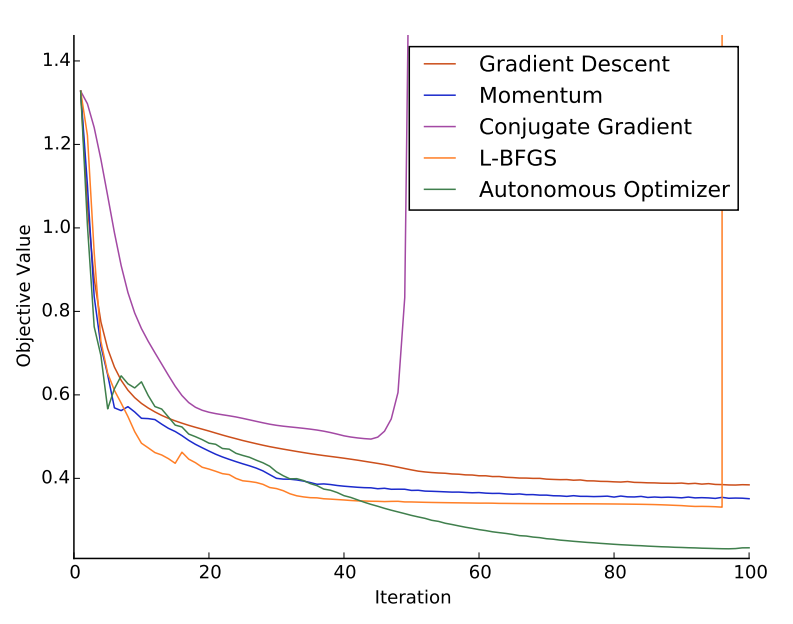
\includegraphics[width=0.5\textwidth]{images/l2o_dnn}

\begin{itemize}
  \item 2-layer DNN with ReLUs
  \item Training datasets for training RL agent:\\ four multivariate Gaussians and sampling 25 points from each
  \begin{itemize}
    \item[$\leadsto$] hard toy problem
  \end{itemize}
\end{itemize}

\end{frame}
%----------------------------------------------------------------------
%----------------------------------------------------------------------
\begin{frame}[c]{Algorithm Control vs. Learning to Learn}


\begin{columns}

\column{0.50\textwidth}

\alert{Algorithm Control:}

\begin{itemize}
  \item Learn to control parameter
  \item Action space: config. space
  \item State space: algorithm state
  \newline
  \item Reward: algorithm performance
\end{itemize}

\column{0.5\textwidth}

\alert{Learning to Learn:}

\begin{itemize}
  \item Learn optimization policy 
  \item Action space: solution space
  \item State space: statistics of previous opt. steps
  \item Reward: solution quality over time
\end{itemize}


\end{columns}


\end{frame}
%----------------------------------------------------------------------
%----------------------------------------------------------------------
\begin{frame}[c]{Learning Goals}

Now, you should be able to \ldots

\begin{itemize}
  \item motivate and define the algorithm control problem
  \item list challenges in algorithm control
  \item explain how reinforcement learning can be used for algorithm control
  \item explain the idea behind learning to   
  \begin{itemize}
    \item learn by gradient descent by gradient descent
    \item optimize black box functions
    \item optimize via reinforcement learning
  \end{itemize}
\end{itemize}

\end{frame}
%----------------------------------------------------------------------
%----------------------------------------------------------------------
\begin{frame}[c]{Teaching Evaluation}

\begin{itemize}
  \item Very important for me (since I'm not yet a professor)
  \pause
  \item Very important for future students attending my lectures
  \pause
  \item I will only get the teaching evaluation if most of you participate!
  \pause
  \item \alert{Please provide constructive feedback!} 
\end{itemize}

\end{frame}
%----------------------------------------------------------------------
%----------------------------------------------------------------------
\begin{frame}[c]{Further Literature---These are links!}

\begin{itemize}
  \item \href{https://www.aaai.org/ocs/index.php/AAAI/AAAI16/paper/download/11763/11767}{Learning Step Size Controllers for Robust Neural Network Training}
  \item \href{https://arxiv.org/abs/1606.04474}{Learning to learn by gradient descent by gradient descent}
  \item \href{http://proceedings.mlr.press/v70/chen17e/chen17e.pdf}{Learning to learn without gradient descent by gradient descent}
  \item \href{https://arxiv.org/pdf/1606.01885.pdf}{Learning to Optimize}
  \item \href{https://arxiv.org/pdf/1703.00441.pdf}{Learning to Optimize Neural Nets}
  \item \href{https://bair.berkeley.edu/blog/2017/09/12/learning-to-optimize-with-rl/}{Blog post on ``Learning to Optimize'' (highly recommended)}
\end{itemize}

\end{frame}
%----------------------------------------------------------------------
